\section{Estudio de la situación actual}

Por suerte, hoy en día existe ya un considerable número de aplicaciones móviles que giran alrededor del mismo eje que lo hace \emph{All for One}, el cuidado y la ayuda de pacientes de Alzheimer. Es de destacar que el Centro de Referencia Estatal de Atención a Personas con Enfermedad de Alzheimer y otras Demencias, abreviado como \textbf{CREA} o CRE Alzheimer, dispone en su página web de un listado muy completo\footnote{\href{https://crealzheimer.imserso.es/crealzheimer\textunderscore01/recursos/apps/index.htm}{https://crealzheimer.imserso.es/crealzheimer\textunderscore01/recursos/apps/index.htm}} (aunque no debidamente actualizado) de las aplicaciones directamente enfocadas en este tema o que lateralmente pueden ser de utilidad en el mismo, categorizándolas según sean de utilidad para cuidadores, pacientes o profesionales; e indicando información de las mismas como una breve descripción o los idiomas en los que se encuentra disponible. 

A continuación se ofrece una selección de las aplicaciones activas más destacables y el cometido para que el son de utilidad a la hora de lidiar con la enfermedad.
\begin{itemize}
    \item \href{https://play.google.com/store/apps/details?id=es.lapisoft.yotecuido}{\textbf{YoTeCuido}}. Información detallada y categorizada para pacientes y cuidadores.
    \item \href{https://play.google.com/store/apps/details?id=com.egm.PharmAlzheimer}{\textbf{Pharma Alzheimer}}. Divulgación e información acerca de la enfermedad.
    \item \href{https://play.google.com/store/apps/details?id=au.com.alzheimersaustraliavic.dementiafriendlyhome}{\textbf{The Dementia-Friendly-Home}}. Información y consejos para adaptar un hogar para que viva una persona con demencia.
    \item \href{https://play.google.com/store/apps/details?id=com.goodbarber.careralzheimer}{\textbf{Cuidador de Alzheimer}}. Comunidad digital para cuidadores.
    \item \href{https://play.google.com/store/apps/details?id=com.alertcops4.app}{\textbf{Alert Cops}}. Aplicación de la Secretaría de Seguridad que permitiría al paciente contactar rápidamente con los cuerpos de seguridad en caso de necesidad.
    \item \href{https://play.google.com/store/apps/details?id=nl.neurodiversiteit.brainy&hl=es_PY}{\textbf{The Brainy App}}. Ejercitación mental para el paciente.
    \item \href{https://play.google.com/store/apps/details?id=mobi.stimulus.stimulushome&hl=es_PY}{\textbf{Stimulus}}. Aplicación para estimulación cognitiva con registro de las sesiones y posibilidad de seguimiento de las mismas por parte de familiares o profesionales.
    \item \href{https://play.google.com/store/apps/details?id=com.imentia.imentiaproffesional2&hl=es_PY}{\textbf{Imentia}}. Otra aplicación de estimulación mental con capacidades multiusuario y de personalización de las sesiones.
    \item \href{https://play.google.com/store/apps/details?id=eu.smartpatient.mytherapy&hl=es_PY}{\textbf{Recordatorio de Medicación}}. Aplicación especializada en alarmas y recordatorios para evitar el olvido de consumo de los fármacos.
\end{itemize}

Todas las aplicaciones anteriores pertenecen al mismo ámbito que el sistema a desarrollar, pero tienen enfoques o utilidades distintas. Ninguna de ellas está enfocada en ofrecer perfiles especializados para pacientes y cuidadores, ni ofrecen las mismas herramientas que pretende ofrecer \emph{All for One}. Son complementos idóneos para los usuarios objetivo del sistema, pero sin superposición con la que nos ocupa.

Por otro lado, en el mercado móvil sí se puede encontrar otro buen número de aplicaciones transversales que ofrecen funcionalidades similares a las que persigue \emph{All for One}, sin pertenecer al mismo ámbito de forma directa. Por ejemplo, aplicaciones de tareas enfocadas a equipos como \href{https://asana.com/es}{\textbf{Asana}} pueden ofrecer la gestión de recordatorios y tareas cooperativa que se intenta ofrecer en el sistema.

En el aspecto de la geolocalización personal es donde se puede encontrar un mayor número de alternativas como \href{https://play.google.com/store/apps/details?id=com.life360.android.safetymapd&hl=es&gl=US}{\textbf{Life360}} (\fref{fig:life365}), \href{https://play.google.com/store/apps/details?id=com.geozilla.family&hl=es&gl=US}{\textbf{Geozilla}} (\fref{fig:geozilla}), \href{https://play.google.com/store/apps/details?id=com.softguard.android.smartpanicsNG&hl=es&gl=US}{\textbf{SmartPanics}} o \href{https://play.google.com/store/apps/details?id=com.safe365.safe365app&hl=es&gl=US}{\textbf{Safe365}}. Todas estas aplicaciones ofrecen un servicio de localización personal de gran nivel con funcionamiento intuitivo y eficaz. Las dos primeras cuentan con un uso muy extendido con varios cientos de miles de descargas debido a su versatilidad para adoptarse a muchas situaciones en las que una funcionalidad de este estilo pueda ser de importancia.

\begin{figure}[H]
    \centering
    \begin{minipage}{0.45\textwidth}
        \centering
        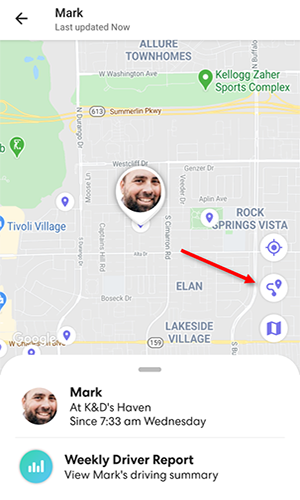
\includegraphics[width=0.45\textwidth]{Introduccion/life360-screenshot.png}
        \caption{Mapa de Life365}
        \label{fig:life365}
    \end{minipage}\hfill
    \begin{minipage}{0.45\textwidth}
        \centering
        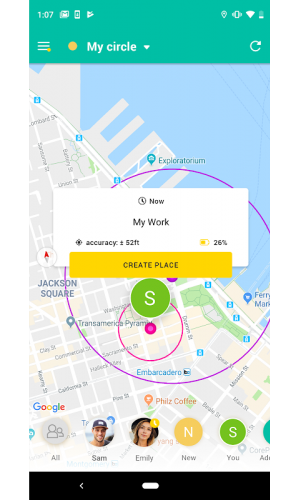
\includegraphics[width=0.45\textwidth]{Introduccion/geozilla-screenshot.png}
        \caption{Mapa de GeoZilla}
        \label{fig:geozilla}
    \end{minipage}
\end{figure}
\vspace{-20pt}
Aún con todo, estas aplicaciones transversales tienen el inconveniente de la carencia del enfoque en la enfermedad. Los gestores de tareas grupales tienden a tener un enfoque profesional para la gestión de equipos de trabajo y con ello tienen un alcance excesivo para el tipo de recordatorios que se deben manejar, complicando su uso para estos menesteres. Las aplicaciones de geolocalización, por otro lado, aunque no están centradas en esta misma enfermedad, sí están diseñadas con necesidades similares en mente y por ello ofrecen una experiencia óptima para el uso que se daría en este ámbito. Lo mismo se puede decir de las aplicaciones de mensajería, que con su diseño generalista también son idóneas para utilizar en los casos que nos ocupan.

Respecto a estos conjuntos de aplicaciones más dedicadas, el aporte que pretende ofrecer \emph{All for One} radica en la comunión de todas estas funcionalidades en un único sistema, evitando configuraciones extra o varias instalaciones para poder contar con todas. Permitiendo a su vez, facilidad en el uso interrelacionado de estas funcionalidades sin excesivos pasos extra y con un canal único de notificaciones común.

\subsection{Evaluación de alternativas}

Dejando a un lado las aplicaciones que ofrecen coincidencias parciales o moderadas podemos pasar a un estudio enfocado en la evaluación de las aplicación con mayores coincidencias y con similutes más directas. Se han seleccionado tres de estas aplicaciones para ofrecer una revisión más dedicada de la que extraer conclusiones que aporten a la hora de diseñar y desarrollar \textbf{All for One}.

\subsubsection{Trusted Elderly Care}

\begin{wrapfigure}[6]{r}{0.2\textwidth}
    \vspace{-20pt}
    \centering
    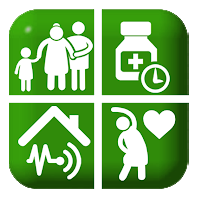
\includegraphics[width=0.15\textwidth]{images/Introduccion/elderly-icon.png}
    \vspace{-17pt}
    \caption{Icono de Elderly Care}
\end{wrapfigure}

Trusted Elderly Care es una aplicación desarrollada por \textbf{LEVStone} disponible en la PlayStore\footnote{\href{https://play.google.com/store/apps/details?id=com.levstone.mobility.trustedelderlycare}{https://play.google.com/store/apps/details?id=com.levstone.mobility.trustedelderlycare}} de Android. La aplicación está enfocada en la monitorización de familiares, especialmente ancianos, y aunque se ofrece de forma gratuita necesita un pago de seis euros para crear los grupos que se usan para el monitoreo, sin embargo, una única cuenta que lo haya adquirido ya permite crear un grupo para todos los familiares. Además de eso, la compañía acepta donaciones en su página web\footnote{\href{https://levstone.com/health-family/trusted-elderly-care/}{https://levstone.com/health-family/trusted-elderly-care/}}.

Como se ha dicho, la aplicación gira en torno a la \textbf{creación de grupos} a los que se deben unir los usuarios para obtener información del resto de usuarios. Entre las funciones que ofrece la aplicación están: elegir un emoji que represente el estado de ánimo, sincronizar la aplicación con sensores y obtener sus lecturas, consultar un mapa con las localizaciones de los usuarios, activar un modo pánico, acceder a los contactos del grupo o crear y consultar tareas entre otras cosas.

La mayoría de estas acciones y otros sucesos relacionados con el usuario como el nivel de carga o el último momento de uso del teléfono móvil \textbf{son notificados al resto de usuarios} del grupo. Sin embargo, el sistema de notificaciones no es instantáneo, la aplicación se debe refrescar para obtener los nuevos cambios en las pantallas o las notificaciones. La aplicación se refresca según el tiempo que el usuario establece en ajustes o usando manualmente el botón de refresco.

\begin{figure}[h]
    \centering
    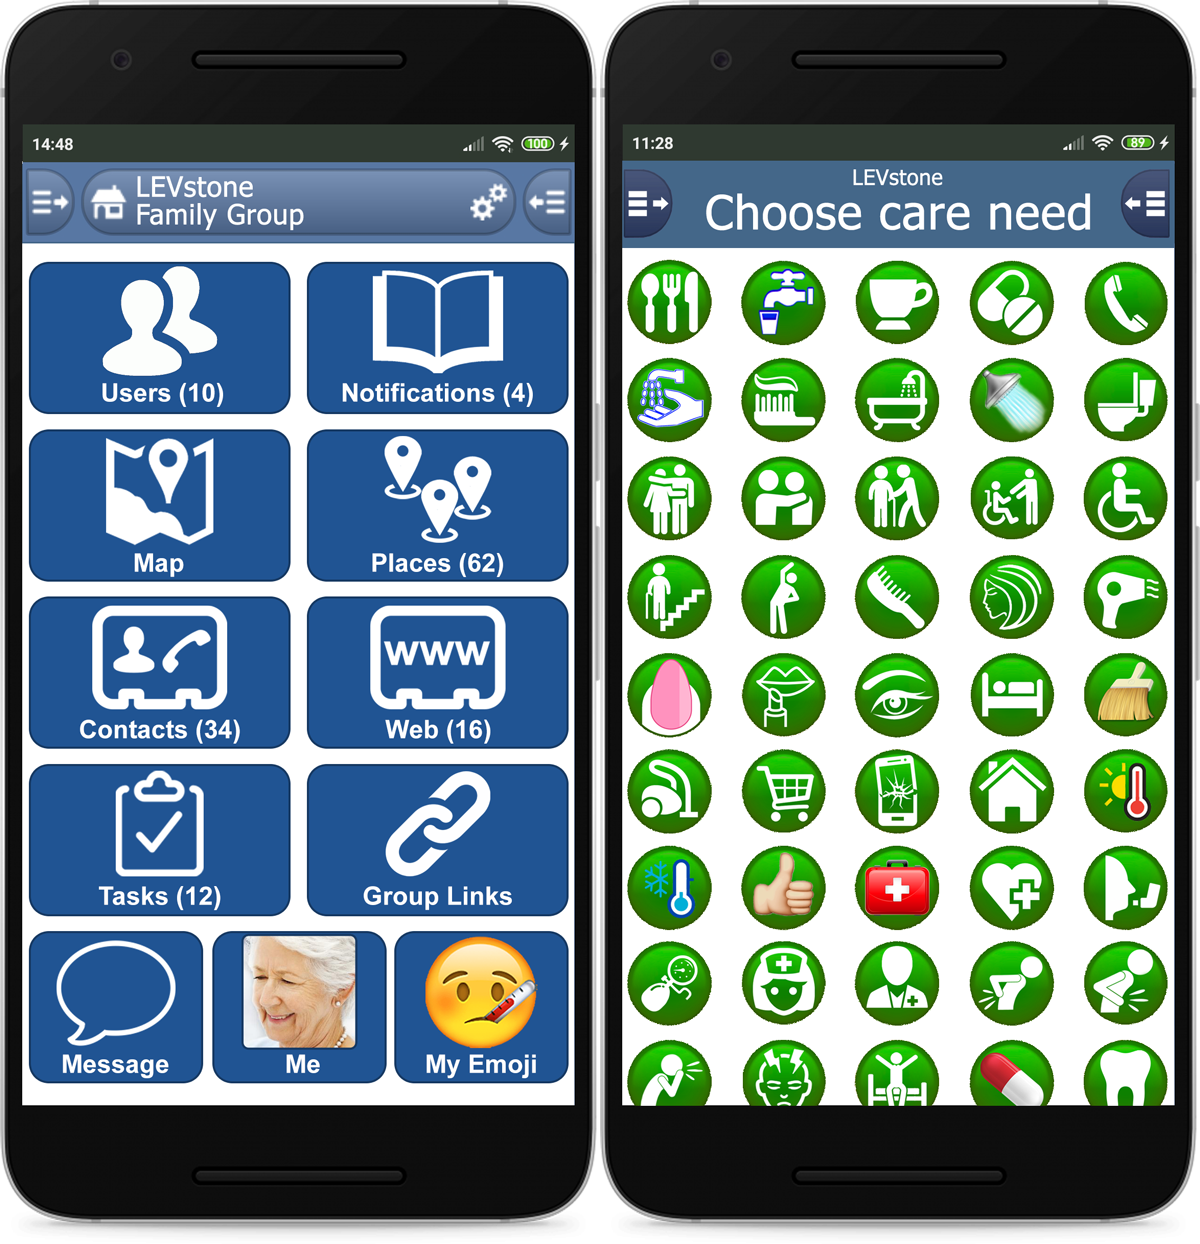
\includegraphics[width=0.5\textwidth]{images/Introduccion/elderly-screenshot.png}
    \caption{Capturas de pantalla de la página web Elderly Care}
\end{figure}

La aplicación permite personalización en bastantes apartados y amplio nivel de detalle y opciones en el uso de sus herramientas. Las tareas que permite crear cuentan con un amplia variedad de campos como establecer la hora y lugar de comienzo y final, el tipo de tarea o los usuarios relacionados con la misma, así como la opción de añadir imágenes o enlaces. En la función de localización ofrece la opción de guardar localizaciones que luego pueden servir, además de para mostrarlas en el mapa, para crear avisos rápidos de estar dirigiéndose hacia el lugar o para ponerlo como lugar donde se llevará a cabo una tarea.

\textbf{El uso de la aplicación es difícil}. La interfaz es ofuscada, está llena de información y no la presenta con iconos o convenciones habituales. Entre otras cosas, los filtros de la ventana de notificaciones están en diferentes botones, nombrados como Usuario o Lugar, que no ofrecen ninguna información de su utilidad. Sin embargo, el mayor problema radica en la navegación, es abstracta y enrevesada, dificultando el acceso al gran número de funciones. Esto es un gran problema de cara a una aplicación pensada para ser usada por gente de avanzada edad, que tienen menos manejo con las tecnologías además de peor visión o memoria entre otras cosas.

\textbf{Virtudes}
\begin{itemize}
    \item Herramienta de tareas muy completa e informativa.
    \item La capacidad de guardar lugares en el mapa.
    \item La vinculación de sensores biométricos.
\end{itemize}

\textbf{Inconvenientes}
\begin{itemize}
    \item Elevado consumo de batería por el monitoreo de recursos.
    \item Navegación ofuscada y enrevesada.
    \item Necesidad de refresco manual para la recepción de nueva información.
    \item Interfaz sobrecargada y poco intuitiva.
\end{itemize}

\subsubsection{Tú y nosotros}

Tú y nosotros (o como aparece en la Play Store\footnote{\href{https://play.google.com/store/apps/details?id=com.tuynosotros.alzheimertyn}{https://play.google.com/store/apps/details?id=com.tuynosotros.alzheimertyn}}, \textbf{Alzheimer App TyN}) es una aplicación desarrollada por A. Calvo. Su principal función es almacenar una ficha con los datos del paciente de Alzheimer y de uno de sus cuidadores (\fref{fig:tyn-ficha}) para que el paciente siempre tenga esa información a mano. Su otra función principal es permitir la creación de recordatorios. Además, \textbf{tiene dos juegos} para el ejercicio mental y un botón para realizar llamadas de emergencia. Como muchas otras aplicaciones también contiene información y enlaces de interés.

Los recordatorios que se pueden crear están compuestos por un nombre que lo define y por una hora a la que se deba recordar. Cuando llega dicha hora \textbf{una notificación es enviada al usuario} con el aviso, de forma que favorece que la pueda llevar a cabo. Además de eso, la notificación se puede marcar como repetible, lo cual hará que esta se notifique diariamente. El usuario también tiene disponible una lista desde la que consultar y eliminar sus recordatorios guardados.

\begin{wrapfigure}[6]{r}{0.2\textwidth}
    \vspace{-20pt}
    \centering
    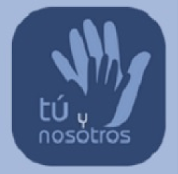
\includegraphics[width=0.15\textwidth]{Introduccion/tyn-icon.png}
    \vspace{-10pt}
    \caption{Icono de Tú y Nosotros}
\end{wrapfigure}

Los juegos ofrecidos por la aplicación son: \textbf{Memoria} (\fref{fig:tyn-memoria}), un juego de parejas con un tablero 4x4 para recordar y juntar parejas de imágenes de conceptos comunes como utensilios, animales o vehículos; y \textbf{Reconoce}, juego en el que se sirven al jugador dos columnas, una con imágenes del mismo tipo que Memoria y otra con los nombres de estos, el jugador debe relacionar cada objeto o animal con el sustantivo que lo nombra.

La aplicación es sencilla de utilizar y muy clara. Sin embargo, \textbf{no cuenta con perfiles ni con interconexión} entre aplicaciones. Es una aplicación con ejecución y persistencia local que no permite la interacción entre cuidadores y pacientes, de hecho, es una aplicación destinada únicamente a los dispositivos de los clientes. Si un cuidador quisiese incluir su información o añadir recordatorios al paciente debería hacerlo desde el móvil del mismo.

\textbf{Virtudes}
\begin{itemize}
    \item Manejo muy sencillo y apto para cualquier usuario.
    \item Aviso por notificación de los recordatorios.
    \item Ficha con información útil para los pacientes.
\end{itemize}

\textbf{Inconvenientes}
\begin{itemize}
    \item No permite ayudar al paciente de forma remota.
    \item Los recordatorios permiten poca información u opciones.
    \item Visualmente le falta claridad en algunos apartados.
\end{itemize}

\vspace{25pt}

\begin{figure}[H]
    \centering
    \begin{minipage}{0.45\textwidth}
        \centering
        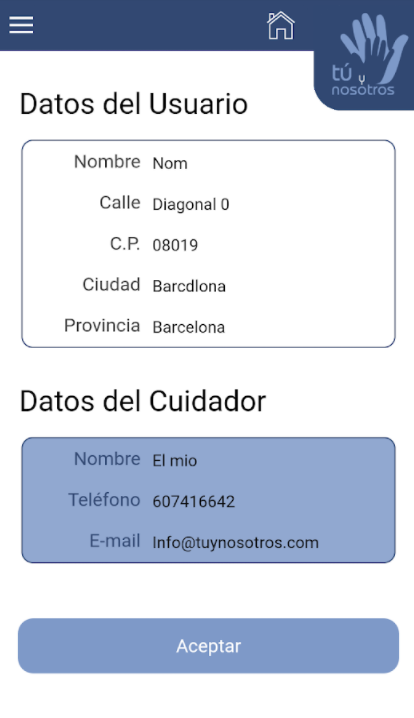
\includegraphics[width=0.45\textwidth]{Introduccion/tyn-screenshot-1.PNG}
        \caption{Ficha de contacto de Tú y Nosotros}
        \label{fig:tyn-ficha}
    \end{minipage}\hfill
    \begin{minipage}{0.45\textwidth}
        \centering
        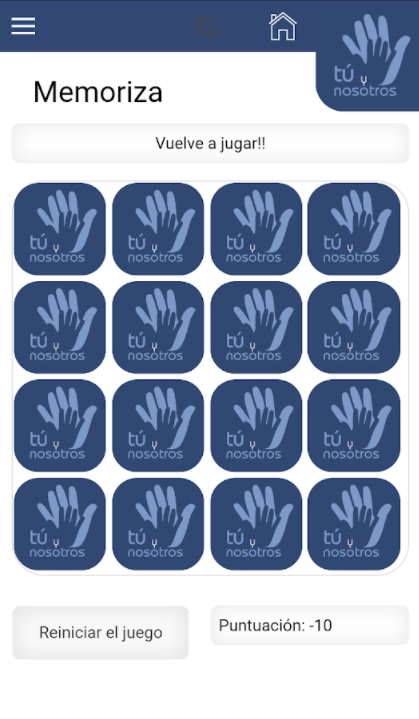
\includegraphics[width=0.45\textwidth]{Introduccion/tyn-screenshot-2.PNG}
        \caption{Juego de memoria de Tú y Nosotros}
        \label{fig:tyn-memoria}
    \end{minipage}
\end{figure}